%!TEX TS-program = xelatex
\documentclass[main]{subfiles}
%这是一个子文件,单独编译时会自动导入main文件的导言区
%这里可以放自定义命令,不会和别人的冲突请放心
%但是不能放newtheorem等高级命令,需要请在群里说
%下面是一些数学命令的简化,可以保留,可以删去,也可以按你的习惯修改
\def\e{\textup{e}}
\def\i{\textup{i}}
\def\T{\textup{T}}
\def\diag{\textup{diag}}
\def\id{\textup{id}}
\newcommand{\toi}[1]{{#1}\to\infty}
\newcommand{\dis}{\displaystyle}
\newcommand{\bv}{\mathrm{BV}}
\newcommand{\ac}{\mathrm{AC}}
\newcommand{\mr}{\mathbb{R}}
\newcommand{\mn}{\mathbb{N}}
\newcommand{\mq}{\mathbb{Q}}
\newcommand{\mz}{\mathbb{Z}}
\newcommand{\rel}{\text{ rel }}
\newcommand{\sgn}{\operatorname{sign}}
\newcommand{\ve}{\varepsilon}
\newcommand{\bs}{\backslash}
\newcommand{\Span}{\operatorname{span}}
\renewcommand{\ll}{\lim\limits}
\renewcommand{\ker}{\operatorname{Ker}}
\renewcommand{\hom}{\operatorname{Hom}}
\renewcommand{\leq}{\leqslant}
\renewcommand{\geq}{\geqslant}
\begin{document}
	\renewcommand{\filename}{26. 多边形外角和}%在这里填你的文件名,避免\label冲突
	%这里开始写你的代码
{\linespread{1.2}
\section{26. 多边形外角和}
\subsection{定理叙述}
	\begin{wrapfigure}{r}{0.2\textwidth}
		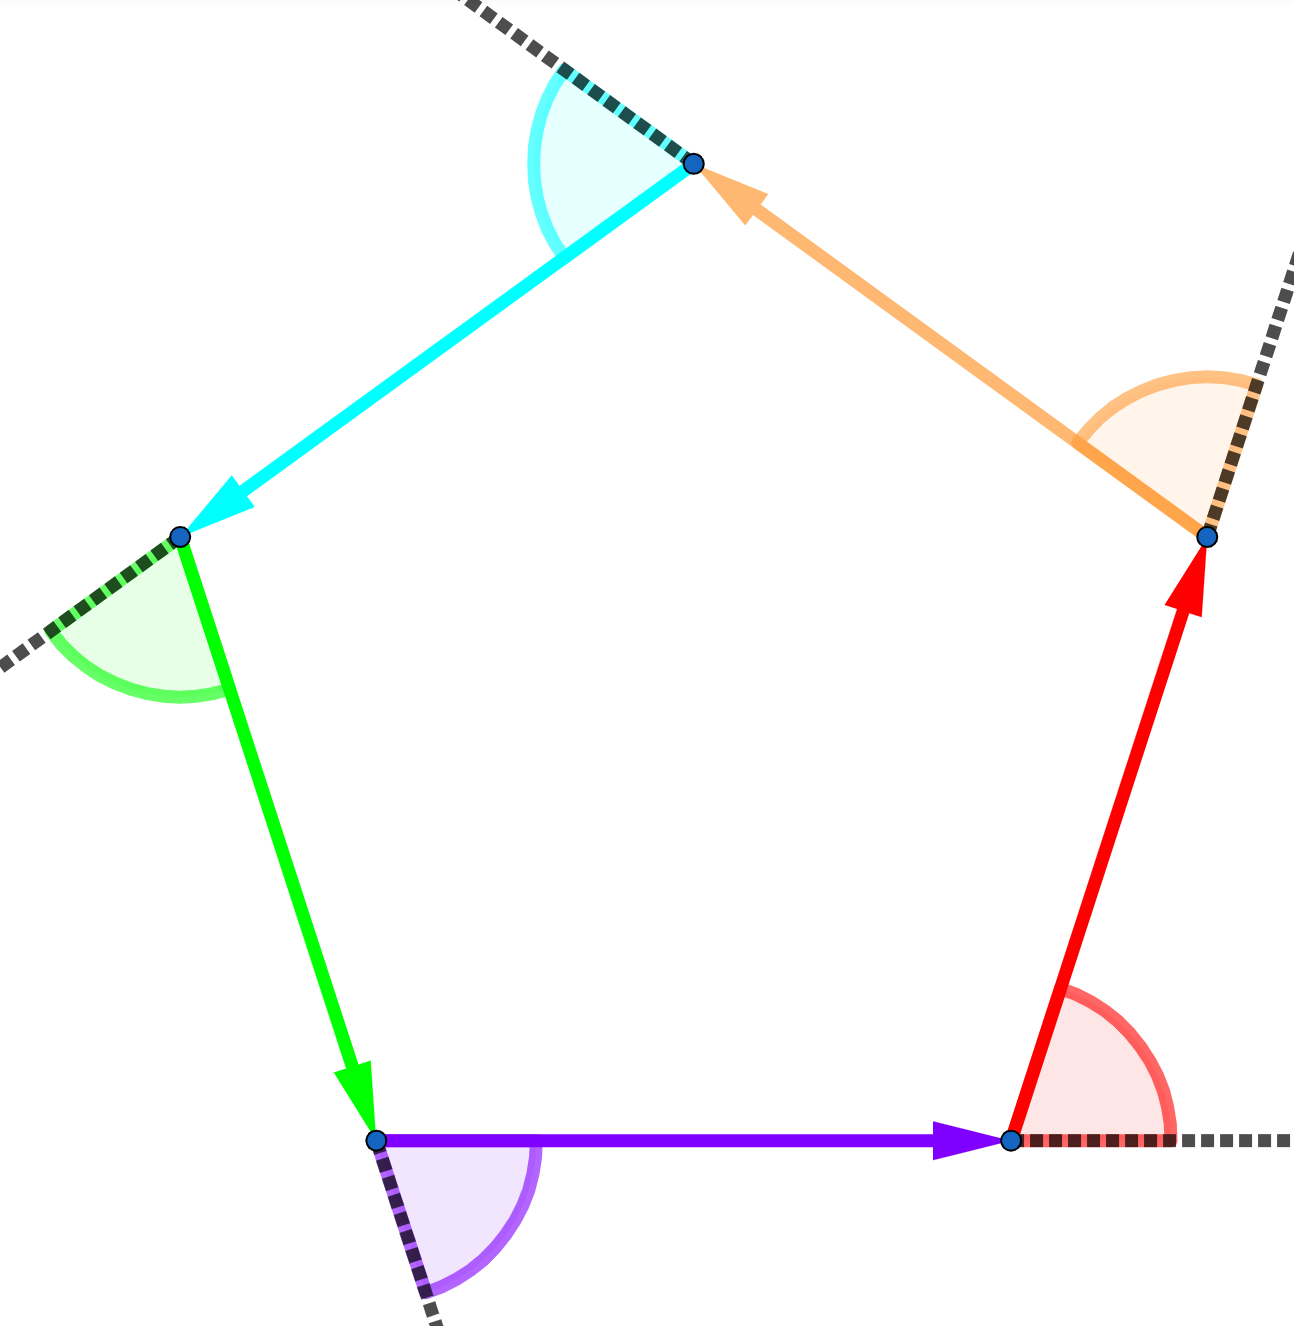
\includegraphics[width=0.19\textwidth]{26_pentagon.png}
		~\\
		~\\
		~\\
		~\\
		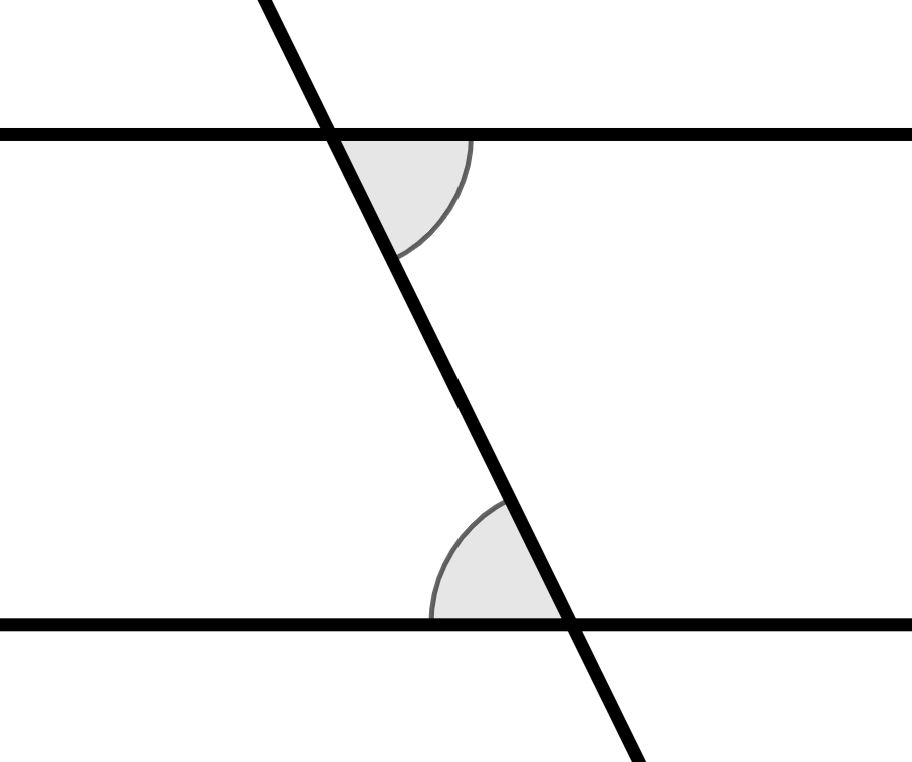
\includegraphics[width=0.19\textwidth]{26_parallel_angles.png}
		~\\
		~\\
		~\\
		~\\
		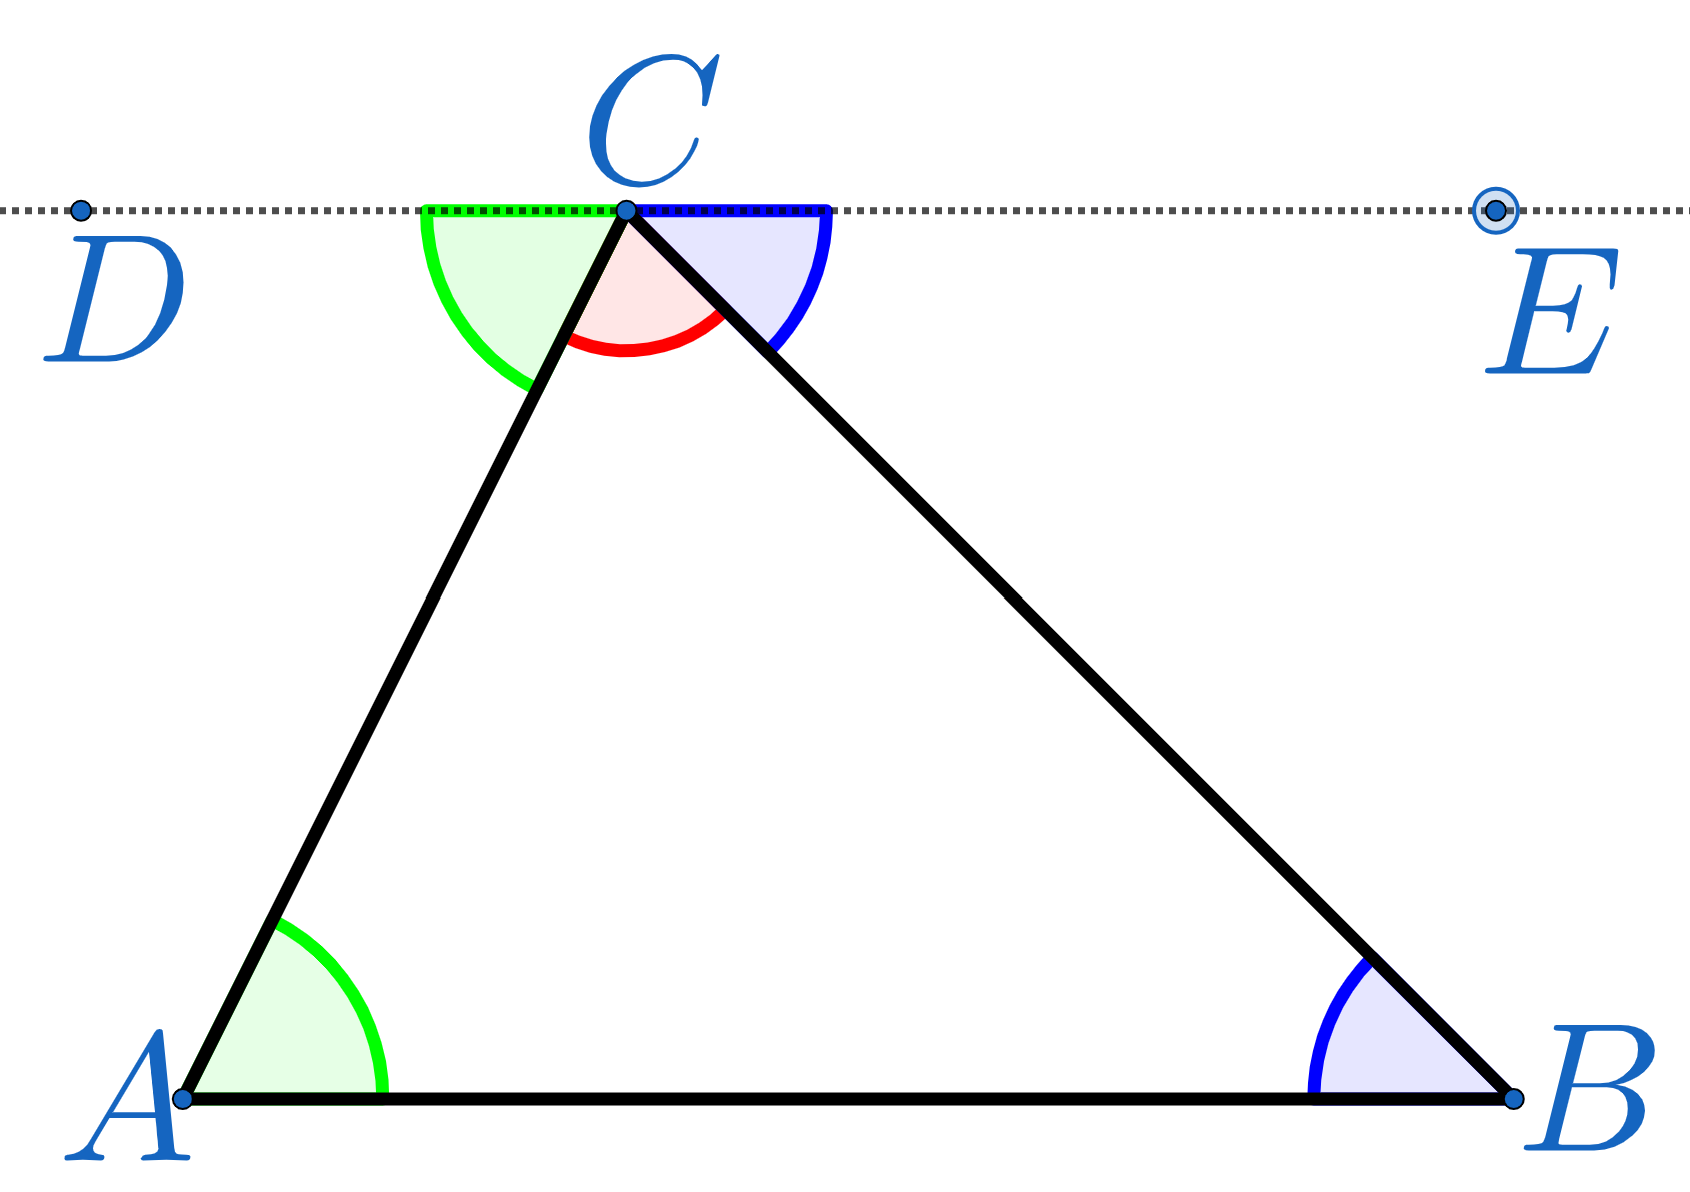
\includegraphics[width=0.19\textwidth]{26_triangle_sum.png}
		~\\
		~\\
		~\\
		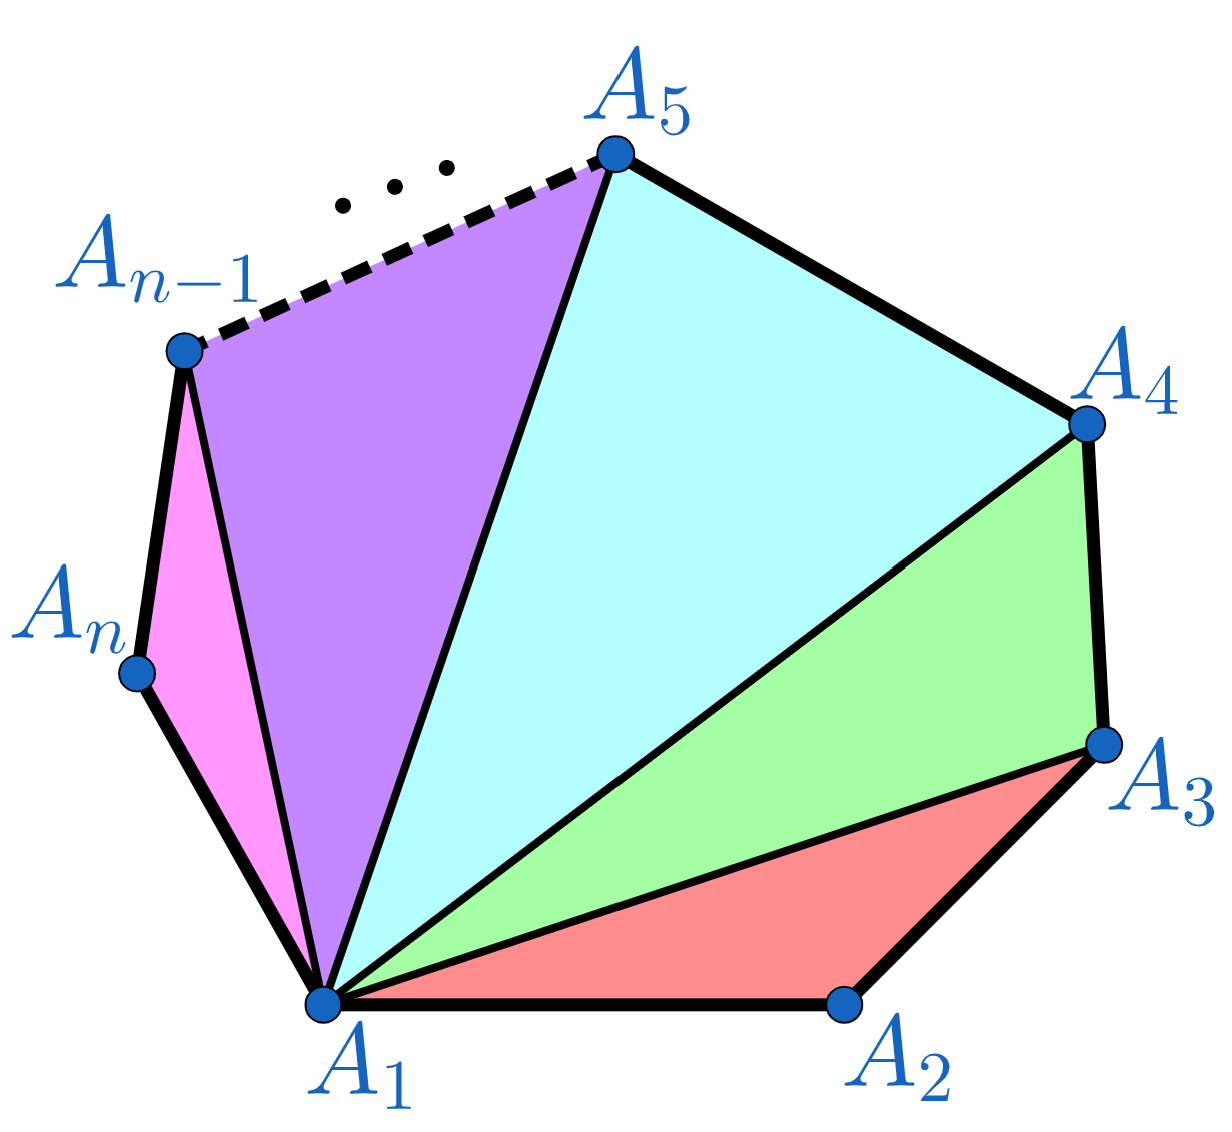
\includegraphics[width=0.19\textwidth]{26_triangulate_convex_polygon.png}
	\end{wrapfigure}
	在平面中, 任意凸多边形的外角和都是$360^{\circ}$.
	
	尽管这一结论看起来过于显然, 从多边形的任一顶点出发, 沿着多边形的边走一圈回到原点, 转过的角之和一定是$360^{\circ}$, 但这一结论并不是平面几何的公理, 仍然需要证明.
\subsection{定理证明}
	\begin{theorem}\label{parallel angles}
		在平面中, 若两直线平行, 则内错角相等.
	\end{theorem}
	\begin{proof}
		该定理就是欧几里得的《几何原本》\cite{Euclid}中的命题1.29, 其中关键之处在于用到了{\kaishu 第五条公理(平行公设)}: 若两条直线都与第三条直线相交, 并且在同一边的内角之和小于两个直角, 则这两条直线在这一边必定相交. 不过近现代的数学家认为欧几里得的公理体系并不是有严格的数理逻辑支撑的公理体系, 尤其是第五条平行公设导致了很多问题. 后来希尔伯特建立了新的平面几何公理体系\cite{Hilbert}, 在这一新体系下证明平行直线内错角相等主要是用到了其{\kaishu 合同(Congruence)公理的第4条}, 大致意思是给定一条射线和张角的大小后可唯一确定另一条射线, 具体证明可参考\cite{Hartshorne}的第113页.
	\end{proof}
	
	\begin{theorem}\label{triangle sum}
		在平面中, 任意三角形的内角和都是$180^{\circ}$.
	\end{theorem}
	\begin{proof}
		欧几里得《几何原本》\cite{Euclid}的命题1.31以及希尔伯特公理体系\cite{Hilbert}的平行公理都认定过直线外一点可以作该直线的平行线. 因此, 如右图所示, 过点$C$可作一条$AB$的平行线$DE$. 由定理\ref{parallel angles}知$\angle A=\angle DCA$, $\angle B=\angle ECB$, 而由于我们作的是一条直线, 天然有$\angle DCA+\angle ACB+\angle ECB=180^{\circ}$, 因此$\angle A+\angle ACB+\angle B=180^{\circ}$, 即$\Delta ABC$的内角和是$180^{\circ}$.
	\end{proof}
	
	\begin{corollary}\label{sum of interior angles}
		在平面中, 任意凸$n$边形($n\geqslant 3$)的内角和都是$(n-2)\cdot 180^{\circ}$.
	\end{corollary}
	\begin{proof}
		由于在凸多边形中连接任意两个顶点的线段都在凸多边形内({\kaishu 为什么? 提示: 连接顶点后分割所得的多边形仍是凸的, 先连接只间隔一个顶点的两个顶点}), 因此凸$n$边形可分割为$n-2$个三角形, 由定理\ref{triangle sum}即得证.
	\end{proof}
	
	\begin{corollary}\label{sum of exterior angles}
		在平面中, 任意凸多边形的外角和都是$360^{\circ}$.
	\end{corollary}
	\begin{proof}
		对于凸多边形而言, 每个顶点处内角、外角之和都是$180^{\circ}$, 那么$n$个顶点处的内外角之和就是$n\cdot 180^{\circ}$; 而推论\ref{sum of interior angles}指出内角和是$(n-2)\cdot 180^{\circ}$, 因此外角和就是$n\cdot 180^{\circ}-(n-2)\cdot 180^{\circ}=360^{\circ}$.
	\end{proof}
	
	\begin{remark}
		\textup{在整个证明过程中, 平面几何的公理至关重要, 否则即使定理\ref{triangle sum}也未必成立(e.g. 球面几何下的三角形).}
	\end{remark}
	
	\begin{remark}
		\textup{\small 推论\ref{sum of interior angles}、\ref{sum of exterior angles}对于一般的多边形(即, 可能有大于$180^{\circ}$的内角)是否成立呢? 笔者尝试过在多边形内取一辅助点来分割多边形和直接将各边平移到一个顶点, 但暂未想出平面几何范围内严谨的证明, 读者可以尝试证明一下:)}
	\end{remark}
	
	{\small
		\begin{thebibliography}{9}
			\bibitem{Euclid} Fitzpatrick, R. (2008). Euclid's elements of geometry.
			\bibitem{Hilbert} Hilbert, D. (1902). The foundations of geometry. Open court publishing Company.
			\bibitem{Hartshorne} Hartshorne, R. (2013). Geometry: Euclid and beyond. Springer Science \& Business Media.
		\end{thebibliography}
	}
}
\end{document}